%! Author = alan
%! Date = 12/22/22



% Preamble
\documentclass[a4paper, 11pt]{article}

% Packages
\usepackage[portuguese]{babel}
\usepackage{amsmath}
\usepackage{graphicx}
\usepackage{setspace}
\usepackage[a4paper, left=2.5cm, right=2.5cm, top=2.5cm, bottom=2.5cm]{geometry}
\usepackage{indentfirst}
\usepackage{listings}
\usepackage{subfig}
\usepackage[utf8]{inputenc}
\usepackage[T1]{fontenc}
\usepackage{array, booktabs, ragged2e}
\usepackage{makecell}
\usepackage{stmaryrd}
\usepackage{siunitx}
\usepackage[siunitx]{circuitikz}
\ctikzset{
    resistors/scale=0.8, % smaller R
    capacitors/scale=0.7, % even smaller C
    diodes/scale=0.6, % small diodes
    transistors/scale=1.2, % bigger BJTs
    transistors/thickness=4,
    transistor circle/relative thickness=0.5,
    bipoles/cuteswitch/thickness=0.25
}
\usepackage{etoolbox}
\AtBeginEnvironment{circuitikz}{%
    \sisetup{mode = text,
        reset-text-family = false,
        reset-text-series = false,
        reset-text-shape = false
    }\sffamily}


\remove{}\usepackage[alf, abnt-emphasize=bf, abnt-thesis-year=both, abnt-repeated-author-omit=no, abnt-last-names=abnt, abnt-etal-cite, abnt-etal-list=3, abnt-etal-text=it, abnt-and-type=e, abnt-doi=doi, abnt-url-package=none, abnt-verbatim-entry=no]{abntex2cite}
\usepackage{textcomp}

% Document
\singlespacing
\begin{document}
	
    \thispagestyle{empty}

\begin{center}
	\begin{figure}[h]
		\centering
		
\includegraphics[width=0.20\linewidth]{pics/ufpa}
		\label{fig:ufpa}
	\end{figure}


	\vspace{1cm}
	\large \uppercase{UNIVERSIDADE FEDERAL DO PARÁ}\\
	\large \uppercase{INSTITUTO DE TECNOLOGIA}\\
	\large \uppercase{BACHARELADO EM ENGENHARIA MECÂNICA}\\
	\vspace{5cm}
	\large \uppercase{NÚCLEO AVANÇADO DE ANÁLISE TENSÕES}\\
	\vspace{1cm}
	\large \uppercase {SISTEMA DE AQUISIÇÃO REMOTA PARA EXTENSOMETRIA} \\
	\vspace{6cm}
	\large {BELÉM/PA \\ 2023}


	%FOLHA DE ROSTO
\end{center}
	\newpage
	\setcounter{page}{1} %comando que redefine a contagem de páginas
	\thispagestyle{empty}

\begin{center}
	LEONARDO DANTAS \\

	\vspace{5cm}

	NÚCLEO AVANÇADO DE ANÁLISE TENSÕES\\
	SISTEMA DE AQUISIÇÃO REMOTA PARA EXTENSOMETRIA\\
\end{center}
	\vspace{5cm}




\singlespacing
\hspace{8cm} % posicionando a caixa de texto
\begin{minipage}{7cm}
	\indent Artigo apresentado para o Núcleo Avançado de Análise de Tensões (NAAT), para o desenvolvimento de nova técnica de aquisição de dados.
\end{minipage}
\vspace{7cm}

\onehalfspacing
\begin{center}
	BELÉM/PA\\
	2023
\end{center}

\newpage
\thispagestyle{empty}
\begin{center}
	ALAN HENRIQUE PEREIRA MIRANDA - MATRICULA:202102140072 \\
	\vspace{5cm}

	Núcleo Avançado de Análise de Tensões\\
	SISTEMA DE AQUISIÇÃO REMOTA PARA EXTENSOMETRIA \\
	\vspace{3cm}

\end{center}
\singlespacing
\hspace{8cm} % posicionando a caixa de texto
\begin{minipage}{7cm}
	\indent Relatório, apresentado à Universidade da Amazônia, como parte das exigências para a obtenção de aprovação disciplinar.\\

	\vspace{2.5cm}

	Belém-PA 21 de maio de 2023 \\
	\vspace{3cm}
\end{minipage}

\onehalfspacing
\begin{center}

	EXAMINADOR\\
	\vspace{2cm}
	\rule{10cm}{0.15mm} \\
	Prof: Dr. Leonardo Dantas \\
	Universidade Federal do Pará - UFPA
\end{center}


    \section{Introdução}
\label{Introducao}

    \indent O circuito proposto é mostrado na Figura 1. Como parâmetros iniciais, determinou-se os valores abaixo.

\begin{figure}[h!]
    \centering
    \begin{circuitikz}
        \draw (0,0)
        (0,0) node[npn, tr circle](Q1){BC548}
        (Q1.base) node[anchor=east]{B}
        (Q1.collector) node[anchor=south]{C}
        (Q1.emitter) node[anchor=north]{E}
        (-2,0) -- (-1,0)
        (-2,0) to [R, l=10K{$\Omega$}] (-2,3.5)
        (0,0.9) to [R, l=3.9K{$\Omega$}] (0,3.5)
        (-2,3.5) -- (0,3.5)
        (-1, 3.5) -- (-1, 4) node[vcc]{$V_{cc}$}
        (-2,0) to [R, l=2.2K{$\Omega$}] (-2,-3.5)
        (-2,-3.5) -- (2, -3.5)
        (0, -0.9) to [eC, l=50<\mu\farad>] (0, -3.5)
        (0, -1) -- (2, -1)
        (2,-1) to[R, l=\SI{820}{$\Omega$}] (2,-3.5)
        (0,-3.5) -- (0,-4.5) node[tlground]{GND}
        (-2,0) to [eC, *-o, l=10<\mu\farad>] (-4,0) node[left]{IN}
        (0,0.9) to [eC, *-o, l=10<\mu\farad>] (2,0.9)  node[right]{OUT}
        ;
    \end{circuitikz}\label{fig:figure}
    \caption{Circuito proposto}

\end{figure}






    \section{Objetivos}
\label{sec:objetivos}

    \indent Este relatório pretende descrever experimentos realizados com um circuito amplificador de um único transistor. O circuito foi anteriormente projetado com auxílio do professor em sala, e os dados obtidos durante os testes serão usados para a montagem do circuito e validação.




    \section{Desenvolvimento}
\label{sec:desenvolvimento}
    \subsection{Circuito}
    \label{sec:circuito}
        \indent O circuito proposto é mostrado na Figura \ref{fig:figure}.
        Como parâmetros iniciais, determinou-se os valores abaixo.\\

        \indent Parâmetros iniciais
        \begin{itemize}
            \item $V_{cc} = 12V$
            \item $R_1 = 10K\Omega$
            \item $R_2 = 3.9K\Omega$
            \item $R_3 = 2.2K\Omega$
            \item $R_4 = 820\Omega$
            \item $C_1 = 10\mu F$
            \item $C_2 = 50\mu F$
        \end{itemize}
        \onehalfspace

        \indent Os parâmetros obtidos foram:
        \begin{itemize}
            \item $I_c = 5 mA$
            \item $V_{ce} = 10V$
            \item $V_{re} = 0.10\cdot V_{cc}$
            \item $V_{cc} = 15\cdot V$
        \end{itemize}

    \indent Ao procurar informações sobre o transistor BC-547, foi possível determinar que trata-se de um transistor NPN de baixa potência, com uma corrente de saturação de $1,8 \cdot 10^{-14} A$ e uma tensão de saturação de $45 V$, mantendo uma faixa de ganho entre $110 hFE$ e $800 hFE$\\

    \indent O transistor BC-547 possui o seguinte diagrama para a polarização de coletor e emissor:
    \begin{figure}[h!]
        \centering
        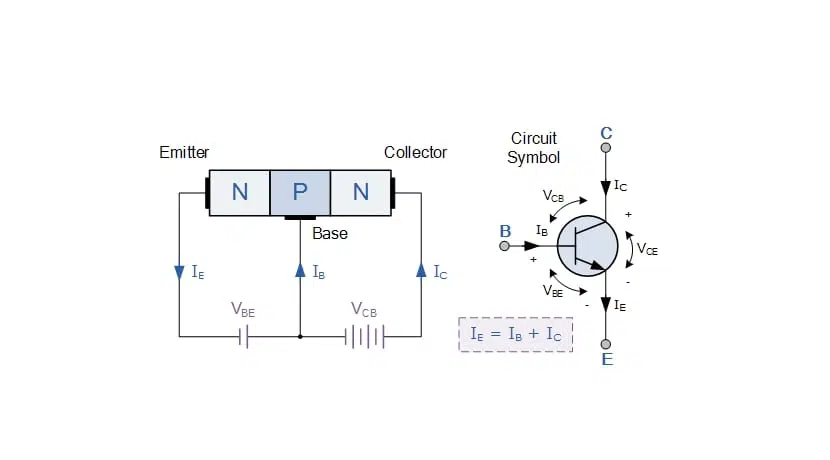
\includegraphics[width=1\textwidth]{pictures/img.png}
        \caption{Diagrama de polarização do transistor BC-547}
        \label{fig:BC547}
    \end{figure}


    \subsection{Procedimentos}
    \label{subsec:procedimentos}
    \indent Para a realização dos testes, foi utilizado um osciloscópio, um multímetro digital e um gerador de sinais.
    O circuito foi montado em uma protoboard com terminais para fonte assimétrica, e os valores de resistores e capacitores foram ajustados para que o circuito funcionasse corretamente.\\

    \indent O circuito foi ligado à fonte de 18V, e o osciloscópio foi conectado ao pino de saída do circuito.
    O gerador de sinais foi conectado ao pino de entrada do circuito, e o multímetro foi conectado ao pino de saída do circuito, sendo configurado para gerar uma onda quadrada com frequência de 1kHz, e o osciloscópio foi configurado para mostrar a onda de saída do circuito.
    O multímetro foi configurado para medir a tensão no pino de saída do circuito, e o osciloscópio foi configurado para mostrar a onda de saída do circuito.\\

    \begin{figure}[h!]
        \centering
        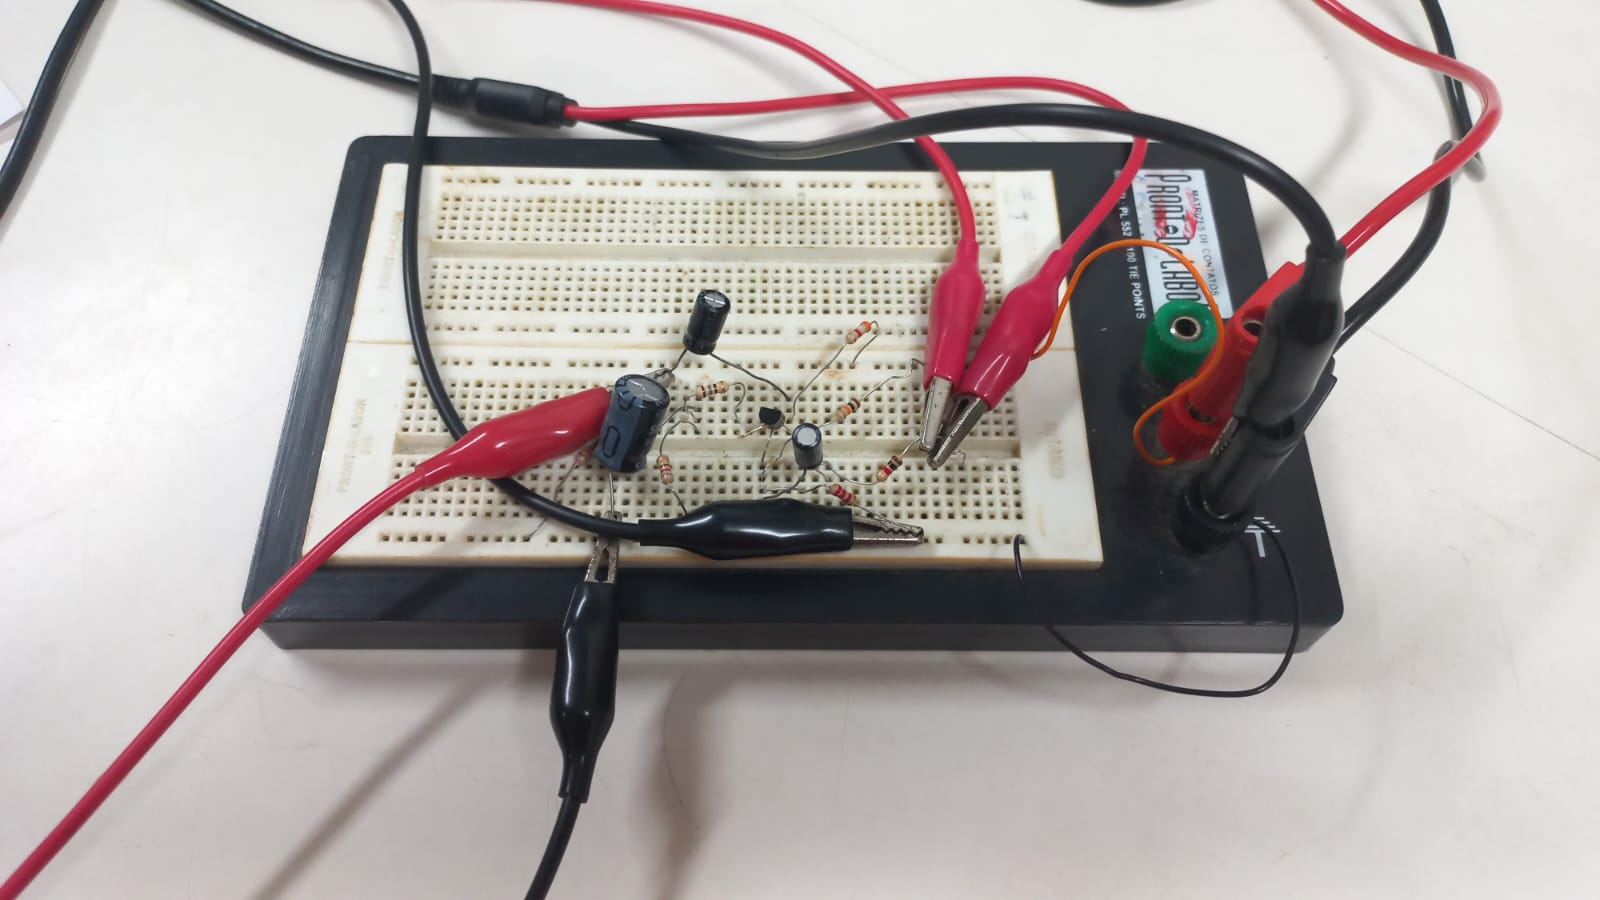
\includegraphics[width=1\textwidth]{pictures/circuito_montado.jpeg}
        \caption{Circuito montado pra testes na protoboard}
        \label{fig:fig1}
    \end{figure}

    \indent No primeiro teste, foi utilizado o gerador de sinais para gerar uma onda quadrada com frequência de 1kHz, e o osciloscópio foi configurado para mostrar a onda de saída do circuito.
     As imputs e outputs do circuito foram, respectivamente $V_{entrada} = 200mV$, $V_{saida} = 1V$, isso para uma alimentação de $10V$ no circuito, essas informações são mostradas na figura a seguir:
    \begin{figure}[h!]
        \centering
        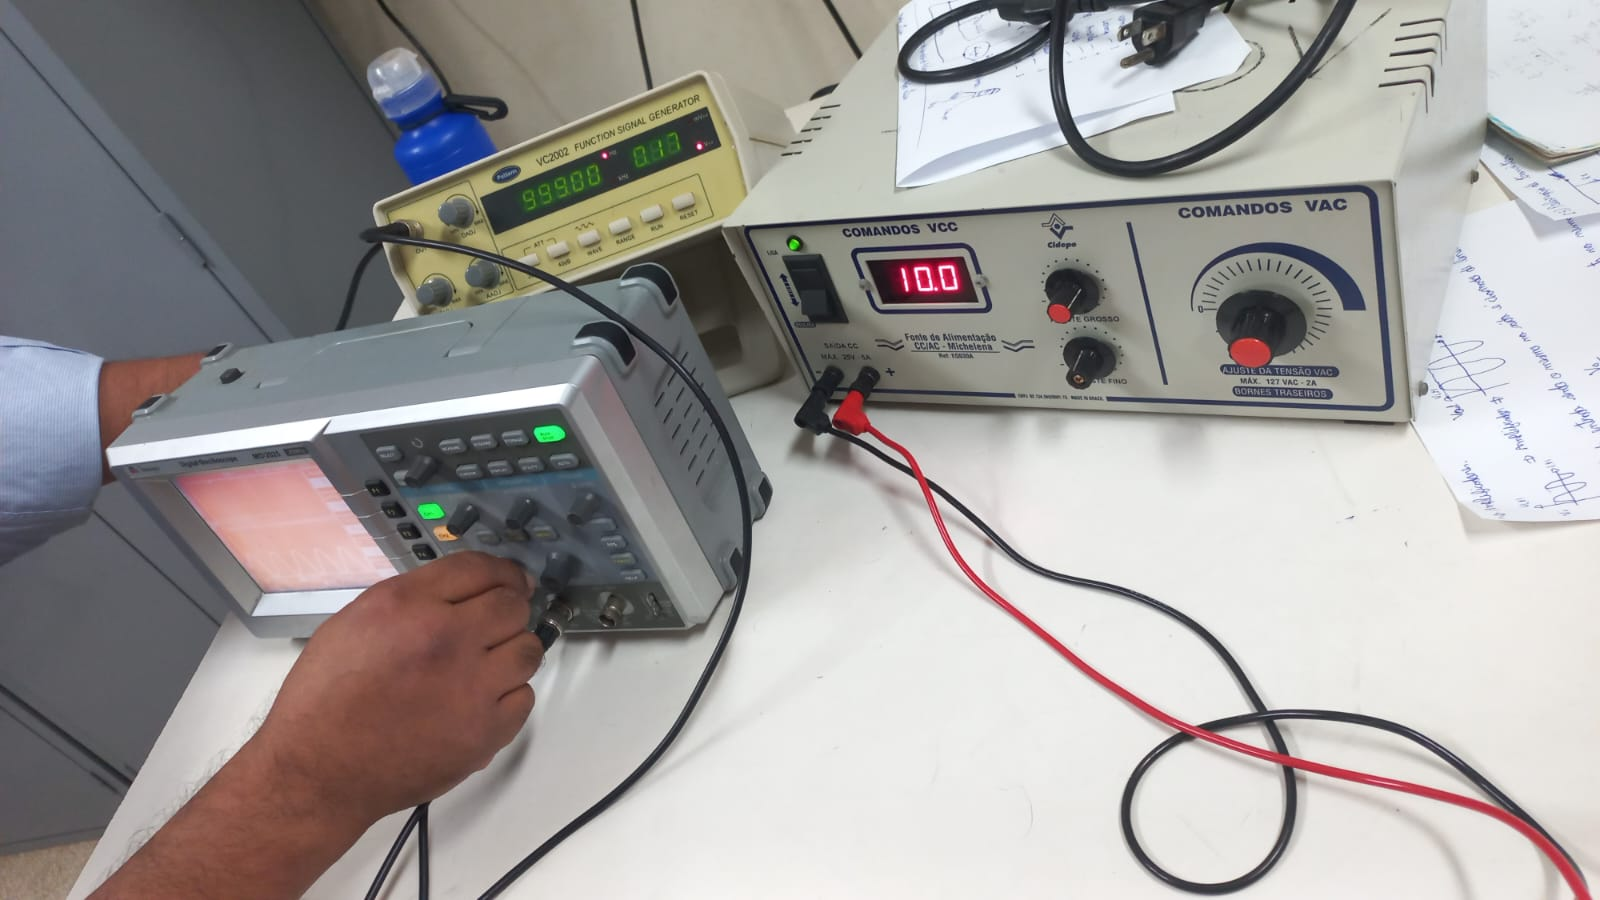
\includegraphics[width=0.4\textwidth]{pictures/bancada de analise.jpeg} \quad
        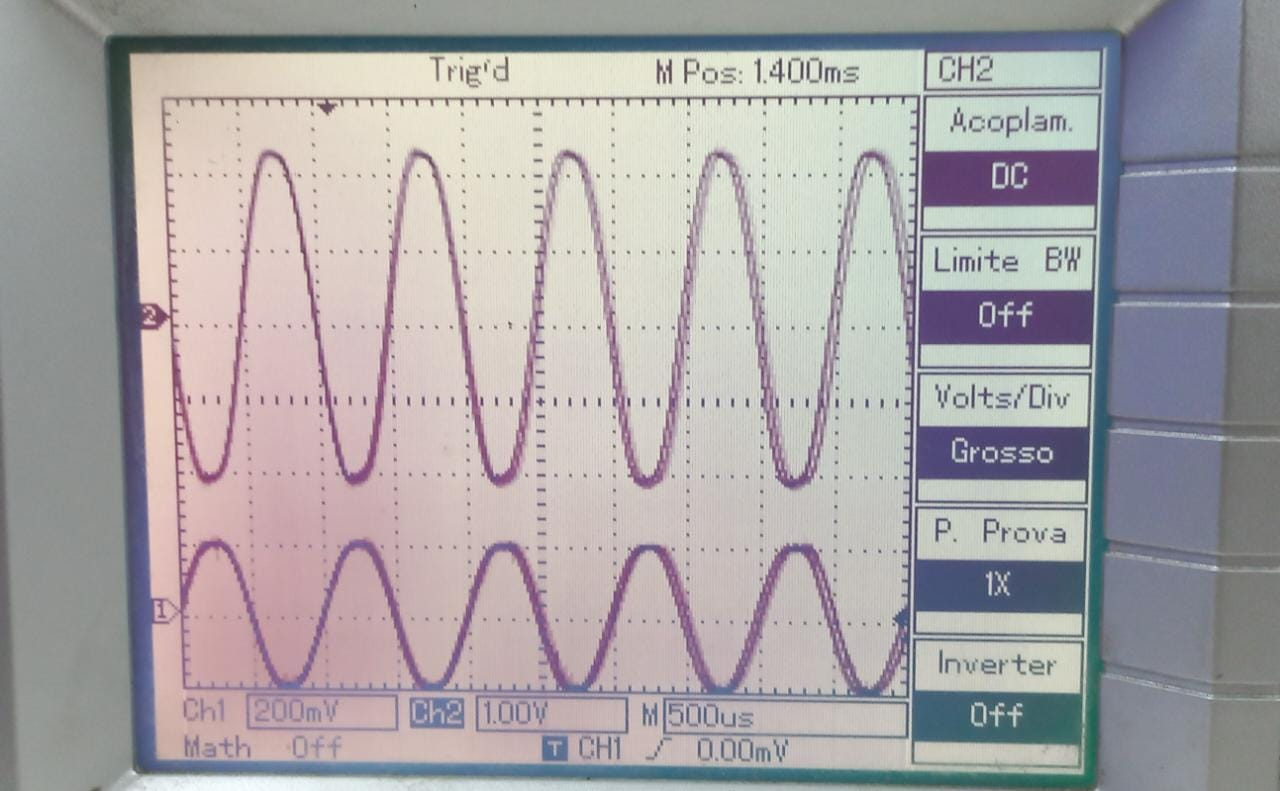
\includegraphics[width=0.4\textwidth]{pictures/osciloscopio teste 1.jpeg}
        \caption{Primeiros Testes de bancada}
        \label{fig:fig2e4}
    \end{figure}

    \indent O ganho observado foi de 5 vezes a entrada, e para o teste em específico, a tensão de saída foi de $1V$.

    \newpage

    \indent No segundo teste, a entrada e saída foram alteradas para $V_{entrada} = 1.14V$ e $V_{saida} = 5.2V$, respectivamente, e o ganho observado foi de 4.56, e para o teste em específico, a tensão em que o sistema foi ligado foi de $18V$.

    \begin{figure}[h!]
        \centering
        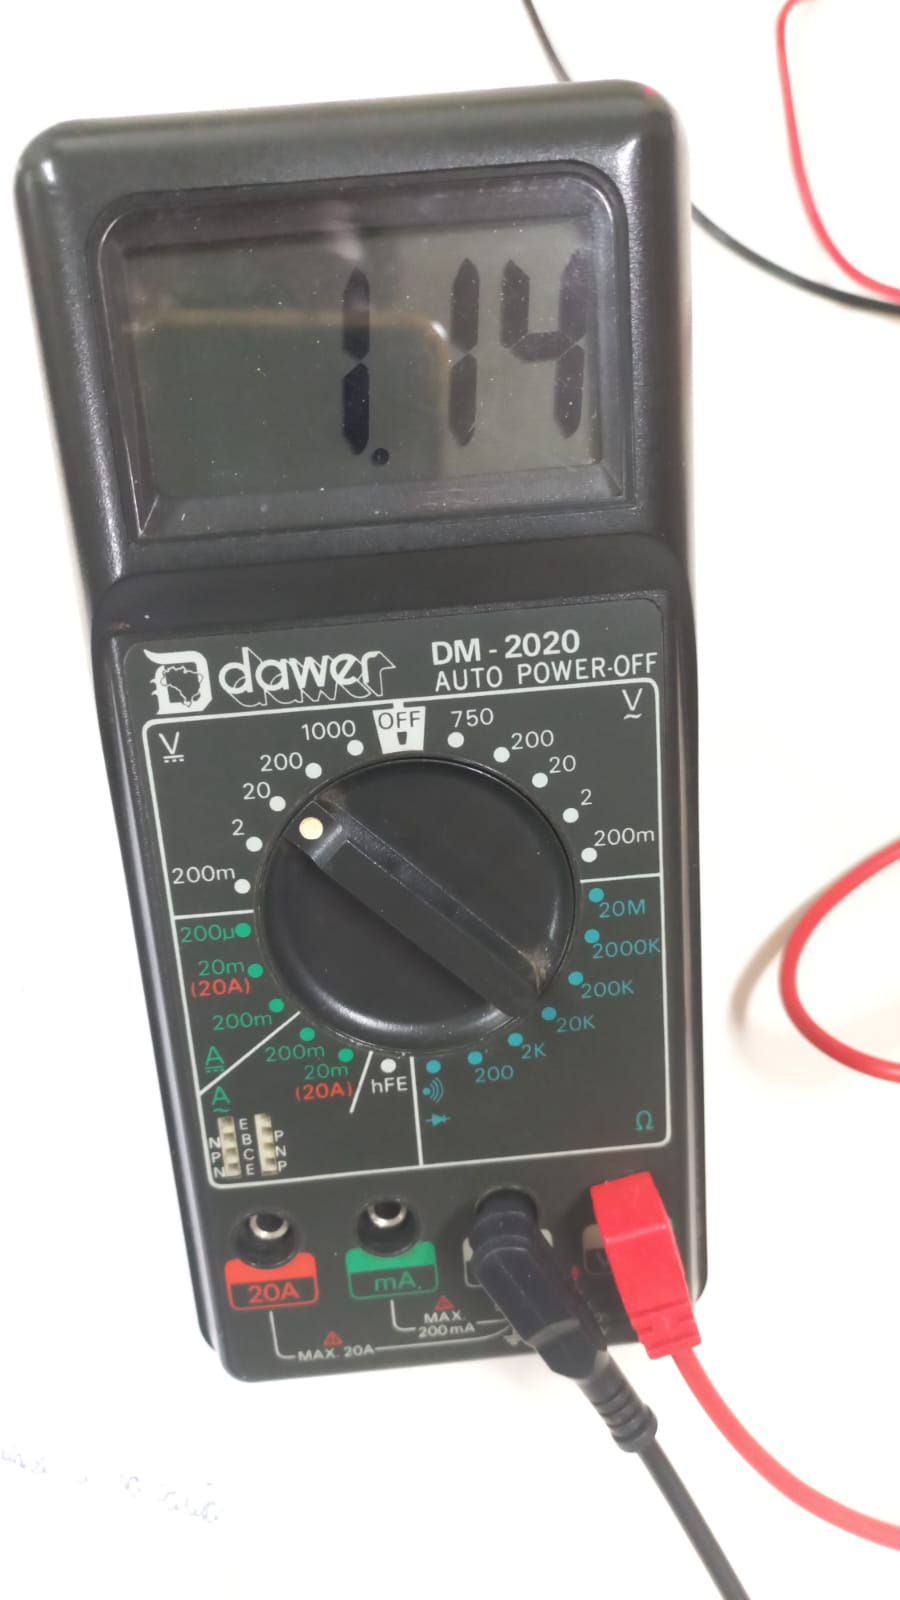
\includegraphics[width=0.4\textwidth]{pictures/mult114.jpeg} \quad
        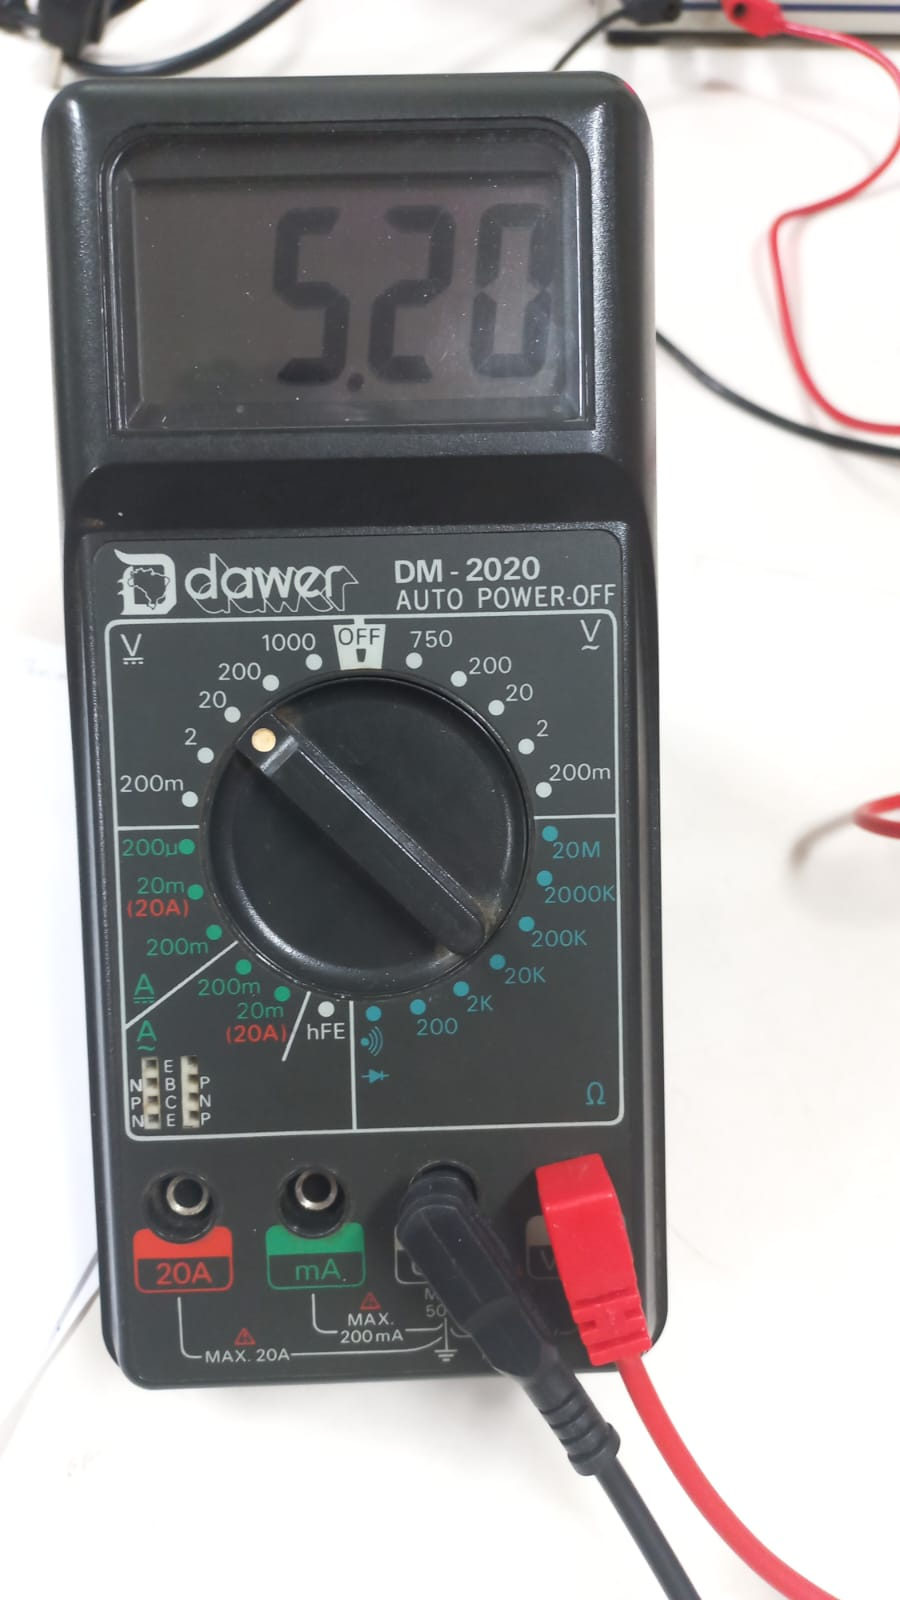
\includegraphics[width=0.4\textwidth]{pictures/mult52.jpeg}
        \caption{Segundos Testes de bancada}
        \label{fig:fig5e6}
    \end{figure}






\end{document}